\usepackage[T1]{fontenc}
\usepackage[utf8]{inputenc}
\usepackage{helvet}
\renewcommand{\familydefault}{\sfdefault}
\usepackage{geometry}
\geometry{paperwidth=6.93in,paperheight=9.11in,inner=0.56in,outer=0.46in,top=0.66in,bottom=0.66in,headheight=14pt}
\usepackage{amsmath}
\usepackage{array}
\usepackage{booktabs}
\usepackage{longtable}
\usepackage{tabularx}
\usepackage{xcolor}
\usepackage{tikz}
\usetikzlibrary{arrows.meta,decorations.pathreplacing,decorations.pathmorphing}
\usepackage{fancyhdr}
\usepackage{titlesec}
\usepackage{enumitem}
\usepackage{etoolbox}
\usepackage{needspace}
\usepackage{hyperref}
\providecommand{\BedrockArchitectureName}{Bedrock}
\providecommand{\BedrockDocumentTitle}{Bedrock Reference}
\providecommand{\BedrockRunningTitle}{REFERENCE}
\providecommand{\BedrockFooterTitle}{BEDROCK ARCHITECTURE}
\hypersetup{colorlinks=true,linkcolor=black,urlcolor=black,pdfauthor={Bedrock Architecture},pdftitle={\BedrockDocumentTitle}}
\makeatletter
\renewcommand{\@pnumwidth}{2.2em}
\renewcommand{\@tocrmarg}{3.0em}
\makeatother
\definecolor{RuleGray}{gray}{0.18}
\definecolor{LightRule}{gray}{0.80}
\setlength{\parindent}{0pt}
\setlength{\parskip}{4pt}
\setlength{\tabcolsep}{2pt}
\sloppy
\emergencystretch=2em
\clubpenalty=10000
\widowpenalty=10000
\displaywidowpenalty=10000
\brokenpenalty=10000
\raggedbottom
\setlist[itemize]{leftmargin=1.0em,itemsep=1pt,topsep=2pt}
\renewcommand{\arraystretch}{1.12}
\pagestyle{fancy}
\fancyhf{}
\fancyhead[LE]{\small \BedrockArchitectureName}
\fancyhead[RO]{\small \BedrockRunningTitle}
\fancyfoot[LE,RO]{\small\thepage}
\fancyfoot[LO,RE]{\small \BedrockFooterTitle}
\renewcommand{\headrulewidth}{0.35pt}
\renewcommand{\footrulewidth}{0pt}
\titleformat{\section}{\large\bfseries\MakeUppercase}{\thesection}{0.7em}{}
\titleformat{\subsection}{\normalsize\bfseries}{\thesubsection}{0.6em}{}
\titlespacing*{\section}{0pt}{1.2em}{0.7em}
\titlespacing*{\subsection}{0pt}{1.0em}{0.45em}
\newcounter{manualfigure}[section]
\newcounter{manualtable}[section]
\renewcommand{\themanualfigure}{\thesection-\arabic{manualfigure}}
\renewcommand{\themanualtable}{\thesection-\arabic{manualtable}}
\newcommand{\manualfield}[2]{%
  \par\noindent\begin{tabularx}{\linewidth}{@{}>{\raggedright\arraybackslash}p{1.46in}X@{}}%
  \textbf{#1} & #2%
  \end{tabularx}\par\vspace{2pt}}
\newcommand{\manualblockfield}[2]{%
  \par\Needspace{0.45in}%
  \begin{description}[style=multiline,leftmargin=1.46in,labelwidth=1.32in,labelsep=0.14in,%
    topsep=0pt,partopsep=0pt,itemsep=0pt,parsep=0pt]%
  \item[\textbf{#1}] #2%
  \end{description}\vspace{2pt}}
\newenvironment{manualraggedblock}{%
  \begingroup\raggedright
}{%
  \par\endgroup}
\newenvironment{manuallongtable}[1]{%
  \begingroup\footnotesize
  \setlength{\LTpre}{2pt}%
  \setlength{\LTpost}{2pt}%
  \begin{longtable}{#1}%
}{%
  \end{longtable}%
  \endgroup}
\newenvironment{manualdenselongtable}[1]{%
  \begingroup\scriptsize
  \setlength{\tabcolsep}{2pt}%
  \setlength{\LTpre}{2pt}%
  \setlength{\LTpost}{2pt}%
  \begin{longtable}{#1}%
}{%
  \end{longtable}%
  \endgroup}
\newenvironment{manualtabular}[1]{%
  \Needspace{1.25in}%
  \begingroup\footnotesize
  \begin{center}%
  \begin{tabular}{#1}%
}{%
  \end{tabular}%
  \end{center}%
  \endgroup}
\newenvironment{manualformblock}[1]{%
  \Needspace{#1}%
  \par\vspace{7pt}\noindent\begin{minipage}{\linewidth}\footnotesize
}{%
  \par\end{minipage}\par}
\newenvironment{manualtikzdiagram}[4]{%
  \begingroup
  \Needspace{#1}%
  \def\manualtikzdiagramcaption{#4}%
  \begin{center}\vspace{3pt}%
  \begin{tikzpicture}[x=#2,y=#3,every node/.style={font=\scriptsize}]%
}{%
  \end{tikzpicture}%
  \manualcaption{\manualtikzdiagramcaption}%
  \end{center}%
  \endgroup}
\newenvironment{manuallistedtikzdiagram}[4]{%
  \begingroup
  \Needspace{#1}%
  \def\manualtikzdiagramcaption{#4}%
  \begin{center}\vspace{3pt}%
  \begin{tikzpicture}[x=#2,y=#3,every node/.style={font=\scriptsize}]%
}{%
  \end{tikzpicture}%
  \manualfigurecaption{\manualtikzdiagramcaption}%
  \end{center}%
  \endgroup}
\newif\ifmanualbitdiagrammeasuring
\newif\ifmanualbitrowmeasuring
\newcount\manualbitdiagramrows
\newcount\manualbitdiagrammaxbits
\newcount\manualbitrowbits
\newcount\manualbitrowindex
\newcount\manualbitfieldx
\newcount\manualbitfieldwidth
\newcommand{\manualbitfield}[2]{%
  \manualbitfieldwidth=#2\relax
  \ifmanualbitrowmeasuring
    \advance\manualbitrowbits by \manualbitfieldwidth
  \else
    \draw ({\the\manualbitfieldx},{\manualbitrowy}) rectangle
      ({\the\numexpr\manualbitfieldx+\manualbitfieldwidth\relax},{\manualbitrowy + 1});
    \node at ({\the\manualbitfieldx + #2/2},{\manualbitrowy + 0.5}) {#1};
    \advance\manualbitfieldx by \manualbitfieldwidth
  \fi}
\newcommand{\manualbitgap}[1]{%
  \manualbitfieldwidth=#1\relax
  \ifmanualbitrowmeasuring
    \advance\manualbitrowbits by \manualbitfieldwidth
  \else
    \advance\manualbitfieldx by \manualbitfieldwidth
  \fi}
\newcommand{\manualbitfieldcode}[2]{\manualbitfield{\texttt{#1}}{#2}}
\newcommand{\manualbitfieldtext}[2]{\manualbitfield{#1}{#2}}
\newcommand{\manualbitlabel}[1]{%
  \ifmanualbitrowmeasuring
  \else
    \pgfmathsetmacro{\manualbitlabelx}{\the\manualbitrowbits-(#1)-0.5}%
    \node[anchor=south] at ({\manualbitlabelx},{\manualbitrowy + 1.18}) {#1};%
  \fi}
\newcommand{\manualbitdefaultlabels}{%
  \node[anchor=south] at (0.5,{\manualbitrowy + 1.18}) {\the\numexpr\manualbitrowbits-1\relax};%
  \node[anchor=south] at ({\the\manualbitrowbits - 0.5},{\manualbitrowy + 1.18}) {0};%
}
\newcommand{\manualbytepairlabels}{%
  \node[anchor=south] at (0.5,{\manualbitrowy + 1.18}) {7};%
  \node[anchor=south] at (7.5,{\manualbitrowy + 1.18}) {0};%
  \node[anchor=south] at (9.5,{\manualbitrowy + 1.18}) {7};%
  \node[anchor=south] at (16.5,{\manualbitrowy + 1.18}) {0};%
  \node[anchor=north] at (4,{\manualbitrowy - 0.16}) {byte 0};%
  \node[anchor=north] at (13,{\manualbitrowy - 0.16}) {byte 1};%
}
\newcommand{\manualbytepairbitlabels}{%
  \node[anchor=south] at (0.5,{\manualbitrowy + 1.18}) {7};%
  \node[anchor=south] at (7.5,{\manualbitrowy + 1.18}) {0};%
  \node[anchor=south] at (9.5,{\manualbitrowy + 1.18}) {7};%
  \node[anchor=south] at (16.5,{\manualbitrowy + 1.18}) {0};%
}
\newcommand{\manualbitrowbody}[4]{%
  \manualbitrowbits=0
  \manualbitrowmeasuringtrue#3\manualbitrowmeasuringfalse
  \ifmanualbitdiagrammeasuring
    \advance\manualbitdiagramrows by 1
    \ifnum\manualbitrowbits>\manualbitdiagrammaxbits
      \manualbitdiagrammaxbits=\manualbitrowbits
    \fi
  \else
    \pgfmathsetmacro{\manualbitrowy}{-2.28*\the\manualbitrowindex}
    \node[anchor=east] at (-0.35,{\manualbitrowy + 0.5}) {#1};
    #2
    \ifnum#4>0
      \ifnum\manualbitrowbits>15
        \foreach \manualbittick in {4,8,...,\the\numexpr\manualbitrowbits-1\relax} {%
          \draw[LightRule] (\manualbittick,\manualbitrowy) -- (\manualbittick,{\manualbitrowy + 1});}
      \fi
    \fi
    \manualbitfieldx=0
    #3
    \advance\manualbitrowindex by 1
  \fi}
\newcommand{\manualbitrowwithlabels}[3]{\manualbitrowbody{#1}{#2}{#3}{1}}
\newcommand{\manualbitfieldrow}[3]{\manualbitrowbody{#1}{#2}{#3}{0}}
\newcommand{\manualbitrow}[2]{\manualbitrowwithlabels{#1}{\manualbitdefaultlabels}{#2}}
\newcommand{\manualrenderbitdiagram}[3]{%
  \begingroup
  \manualbitdiagramrows=0
  \manualbitdiagrammaxbits=0
  \manualbitdiagrammeasuringtrue#2\manualbitdiagrammeasuringfalse
  \pgfmathsetmacro{\manualbitdiagramneedspace}{0.90 + 0.50*\the\manualbitdiagramrows}
  \pgfmathsetmacro{\manualbitdiagramxscale}{min(0.30, 4.70/\the\manualbitdiagrammaxbits)}
  \Needspace{\manualbitdiagramneedspace in}%
  \begin{center}\vspace{3pt}%
  \begin{tikzpicture}[x=\manualbitdiagramxscale in,y=0.22in,every node/.style={font=\scriptsize}]%
  \manualbitrowindex=0
  #2
  \end{tikzpicture}%
  #3{#1}%
  \end{center}%
  \endgroup}
\NewDocumentEnvironment{manualbitdiagram}{m +b}{%
  \manualrenderbitdiagram{#1}{#2}{\manualcaption}%
}{}
\NewDocumentEnvironment{manuallistedbitdiagram}{m +b}{%
  \manualrenderbitdiagram{#1}{#2}{\manualfigurecaption}%
}{}
\newif\ifmanualformatdiagrammeasuring
\newif\ifmanualformatrowmeasuring
\newcount\manualformatdiagramrows
\newcount\manualformatdiagrammaxunits
\newcount\manualformatrowbits
\newcount\manualformatrowunits
\newcount\manualformatrowindex
\newcount\manualformatfieldbits
\newcount\manualformatfieldunits
\newcount\manualformatfieldx
\newcount\manualformatfieldhigh
\newcount\manualformatrowlow
\newcount\manualformatfieldminunits
\newcommand{\manualformatfield}[2]{%
  \manualformatfieldbits=#2\relax
  \manualformatfieldunits=\manualformatfieldbits
  \ifnum\manualformatfieldunits<\manualformatfieldminunits
    \manualformatfieldunits=\manualformatfieldminunits
  \fi
  \ifmanualformatrowmeasuring
    \advance\manualformatrowbits by \manualformatfieldbits
    \advance\manualformatrowunits by \manualformatfieldunits
  \else
    \ifnum\manualformatfieldhigh>\manualformatrowlow
      \ifnum\manualformatfieldbits=1
        \node[anchor=south east] at ({\the\numexpr\manualformatfieldx+\manualformatfieldunits\relax},{\manualformatrowy + 1.18}) {\the\manualformatfieldhigh};
      \else
        \node[anchor=south] at ({\the\manualformatfieldx},{\manualformatrowy + 1.18}) {\the\manualformatfieldhigh};
      \fi
    \fi
    \draw ({\the\manualformatfieldx},{\manualformatrowy}) rectangle
      ({\the\numexpr\manualformatfieldx+\manualformatfieldunits\relax},{\manualformatrowy + 1});
    \node at ({\the\manualformatfieldx + \the\manualformatfieldunits/2},{\manualformatrowy + 0.5}) {#1};
    \advance\manualformatfieldx by \manualformatfieldunits
    \advance\manualformatfieldhigh by -\manualformatfieldbits
  \fi}
\newcommand{\manualformatfieldcode}[2]{\manualformatfield{\texttt{#1}}{#2}}
\newcommand{\manualformatrowrange}[4]{%
  \manualformatrowbits=0
  \manualformatrowunits=0
  \manualformatrowmeasuringtrue#4\manualformatrowmeasuringfalse
  \ifmanualformatdiagrammeasuring
    \advance\manualformatdiagramrows by 1
    \ifnum\manualformatrowunits>\manualformatdiagrammaxunits
      \manualformatdiagrammaxunits=\manualformatrowunits
    \fi
  \else
    \pgfmathsetmacro{\manualformatrowy}{-2.08*\the\manualformatrowindex}
    \node[anchor=east] at (-0.35,{\manualformatrowy + 0.5}) {#1};
    \manualformatfieldx=0
    \manualformatrowlow=#3\relax
    \manualformatfieldhigh=#2\relax
    #4
    \node[anchor=south east] at ({\the\manualformatfieldx},{\manualformatrowy + 1.18}) {#3};
    \advance\manualformatrowindex by 1
  \fi}
\newcommand{\manualformatrow}[2]{%
  \manualformatrowbits=0
  \manualformatrowunits=0
  \manualformatrowmeasuringtrue#2\manualformatrowmeasuringfalse
  \manualformatrowrange{#1}{\number\numexpr\manualformatrowbits-1\relax}{0}{#2}}
\newcommand{\manualrenderformatdiagram}[4]{%
  \begingroup
  \manualformatfieldminunits=#2\relax
  \manualformatdiagramrows=0
  \manualformatdiagrammaxunits=0
  \manualformatdiagrammeasuringtrue#3\manualformatdiagrammeasuringfalse
  \pgfmathsetmacro{\manualformatdiagramneedspace}{0.80 + 0.45*\the\manualformatdiagramrows}
  \pgfmathsetmacro{\manualformatdiagramxscale}{min(0.30, 4.58/\the\manualformatdiagrammaxunits)}
  \Needspace{\manualformatdiagramneedspace in}%
  \begin{center}\vspace{3pt}%
  \begin{tikzpicture}[x=\manualformatdiagramxscale in,y=0.22in,every node/.style={font=\scriptsize}]%
  \manualformatrowindex=0
  #3
  \end{tikzpicture}%
  #4{#1}%
  \end{center}%
  \endgroup}
\NewDocumentEnvironment{manualformatdiagram}{m m +b}{%
  \manualrenderformatdiagram{#1}{#2}{#3}{\manualcaption}%
}{}
\NewDocumentEnvironment{manuallistedformatdiagram}{m m +b}{%
  \manualrenderformatdiagram{#1}{#2}{#3}{\manualfigurecaption}%
}{}
\newif\ifmanualbyteordermeasuring
\newcount\manualbyteordercells
\newcount\manualbyteordercellindex
\newcommand{\manualbytecell}[2]{%
  \ifmanualbyteordermeasuring
    \advance\manualbyteordercells by 1
  \else
    \draw ({\the\manualbyteordercellindex},0) rectangle
      ({\the\numexpr\manualbyteordercellindex+1\relax},1);
    \node at ({\the\manualbyteordercellindex + 0.5},0.62) {#1};
    \node[anchor=north] at ({\the\manualbyteordercellindex + 0.5},-0.04) {\texttt{#2}};
    \advance\manualbyteordercellindex by 1
  \fi}
\newcommand{\manualrenderbyteorderdiagram}[8]{%
  \begingroup
  \manualbyteordercells=0
  \manualbyteordermeasuringtrue#7\manualbyteordermeasuringfalse
  \pgfmathsetmacro{\manualbyteorderxscale}{min(0.72, 4.70/\the\manualbyteordercells)}
  \Needspace{1.35in}%
  \begin{center}\vspace{3pt}%
  \begin{tikzpicture}[x=\manualbyteorderxscale in,y=0.34in,every node/.style={font=\scriptsize}]%
  \manualbyteordercellindex=0
  #7
  \node[anchor=east] at (-0.15,0.62) {#2};
  \node[anchor=east] at (-0.15,-0.20) {#3};
  \draw[->] (0,-0.70) -- node[below] {#4} (\the\manualbyteordercells,-0.70);
  \node[anchor=west] at (0,1.22) {#5};
  \node[anchor=east] at (\the\manualbyteordercells,1.22) {#6};
  \end{tikzpicture}%
  #8{#1}%
  \end{center}%
  \endgroup}
\NewDocumentEnvironment{manualbyteorderdiagram}{m m m m m m +b}{%
  \manualrenderbyteorderdiagram{#1}{#2}{#3}{#4}{#5}{#6}{#7}{\manualcaption}%
}{}
\NewDocumentEnvironment{manuallistedbyteorderdiagram}{m m m m m m +b}{%
  \manualrenderbyteorderdiagram{#1}{#2}{#3}{#4}{#5}{#6}{#7}{\manualfigurecaption}%
}{}
\newif\ifmanualstackframemeasuring
\newcount\manualstackframerows
\newcount\manualstackframerowindex
\newcommand{\manualstackframewidth}{3.25}
\newcommand{\manualstackframerowheight}{0.50}
\newcommand{\manualstackframeslotbody}[4]{%
  \ifmanualstackframemeasuring
    \advance\manualstackframerows by 1
  \else
    \pgfmathsetmacro{\manualstackframey}{-\manualstackframerowheight*\the\manualstackframerowindex}%
    \pgfmathsetmacro{\manualstackframemidy}{\manualstackframey - \manualstackframerowheight/2}%
    \ifnum#4>0
      \node[anchor=east] at (-0.44,\manualstackframemidy) {SP};%
      \draw[->] (-0.40,\manualstackframemidy) -- (-0.02,\manualstackframemidy);%
    \else
      \node[anchor=east] at (-0.08,\manualstackframemidy) {\texttt{#1}};%
    \fi
    \ifnum#3>0
      \draw[densely dashed] (0,{\manualstackframey - \manualstackframerowheight}) -- (0,\manualstackframey) -- (\manualstackframewidth,\manualstackframey) -- (\manualstackframewidth,{\manualstackframey - \manualstackframerowheight});%
    \else
      \draw (0,\manualstackframey) rectangle (\manualstackframewidth,{\manualstackframey - \manualstackframerowheight});%
    \fi
    \node at ({\manualstackframewidth/2},\manualstackframemidy) {#2};%
    \advance\manualstackframerowindex by 1
  \fi}
\newcommand{\manualstackframeslot}[2]{\manualstackframeslotbody{#1}{#2}{0}{0}}
\newcommand{\manualstackframespslot}[2]{\manualstackframeslotbody{#1}{#2}{0}{1}}
\newcommand{\manualstackframepayload}[2]{\manualstackframeslotbody{#1}{#2}{1}{0}}
\newcommand{\manualrenderstackframediagram}[3]{%
  \begingroup
  \manualstackframerows=0
  \manualstackframemeasuringtrue#2\manualstackframemeasuringfalse
  \pgfmathsetmacro{\manualstackframeneedspace}{0.95 + 0.18*\the\manualstackframerows}%
  \Needspace{\manualstackframeneedspace in}%
  \begin{center}\vspace{3pt}%
  \begin{tikzpicture}[x=1in,y=0.30in,every node/.style={font=\scriptsize}]%
  \node[anchor=south] at (0.00,0.26) {63};%
  \node[anchor=south] at (\manualstackframewidth,0.26) {0};%
  \manualstackframerowindex=0
  #2
  \end{tikzpicture}%
  #3{#1}%
  \end{center}%
  \endgroup}
\NewDocumentEnvironment{manualstackframediagram}{m +b}{%
  \manualrenderstackframediagram{#1}{#2}{\manualcaption}%
}{}
\NewDocumentEnvironment{manuallistedstackframediagram}{m +b}{%
  \manualrenderstackframediagram{#1}{#2}{\manualfigurecaption}%
}{}
\newcommand{\manualifempty}[3]{%
  \if\relax\detokenize{#1}\relax
    #2%
  \else
    #3%
  \fi}
\newcommand{\manualeaflowstart}[2]{%
  \begingroup
  \Needspace{#1}%
  \def\manualeaflowcaption{#2}%
  \begin{center}\vspace{2pt}%
  \begin{tikzpicture}[x=1in,y=1in,every node/.style={font=\scriptsize},>=stealth]%
}
\newcommand{\manualeaflowend}{%
  \end{tikzpicture}%
  \manualcaption{\manualeaflowcaption}%
  \end{center}%
  \endgroup}
\newcommand{\manualeaflowrowlabel}[4]{%
  \node[anchor=west] at (0.02,#2) {#1};
  \draw (#3,#2) -- (#4,#2);}
\newcommand{\manualeaflowbox}[6]{%
  \node[draw,align=center,minimum width=#4in,minimum height=0.26in] (#1) at (#2,#3) {#5};
  \ifnum#6>0
    \node[anchor=south] at ({#2 - #4/2},{#3 + 0.16}) {63};
    \node[anchor=south] at ({#2 + #4/2},{#3 + 0.16}) {0};
  \fi}
\newcommand{\manualeaflowlabeledbox}[7]{%
  \pgfmathsetmacro{\manualeaflowleft}{#4 - #5/2}%
  \manualeaflowrowlabel{#1}{#3}{1.55}{\manualeaflowleft}%
  \manualeaflowbox{#2}{#4}{#3}{#5}{#6}{#7}}
\newcommand{\manualeaflowcircle}[4]{%
  \node[draw,circle,inner sep=0pt,minimum size=0.27in] (#1) at (#2,#3) {#4};}
\newcommand{\manualeaflowmemorytail}[4]{%
  \manualeaflowlabeledbox{MEMORY}{mem}{#2}{#3}{#4}{OPERAND}{0}%
  \draw[->] (#1.south) -- node[midway,right] {POINTS TO} (mem.north);}
\newcommand{\manualeadirectflow}[4]{%
  \manualeaflowstart{1.55in}{#1}%
  \manualeaflowlabeledbox{#2}{reg}{0.18}{3.82}{3.05}{#3}{1}%
  \manualeaflowlabeledbox{OPERAND}{operand}{-0.62}{3.82}{3.05}{#4}{0}%
  \draw[->] (reg.south) -- (operand.north);%
  \manualeaflowend}
\newcommand{\manualeaimmediateflow}[3]{%
  \manualeaflowstart{1.55in}{#1}%
  \manualeaflowlabeledbox{IMMEDIATE DATA}{imm}{0.20}{3.82}{3.05}{#2}{1}%
  \manualeaflowlabeledbox{OPERAND}{operand}{-0.62}{3.82}{3.05}{#3}{0}%
  \draw[->] (imm.south) -- (operand.north);%
  \manualeaflowend}
\newcommand{\manualeasimplememoryflow}[4]{%
  \manualeaflowstart{2.10in}{#1}%
  \manualeaflowlabeledbox{#2}{src}{0.18}{3.82}{3.05}{#3}{1}%
  \manualeaflowlabeledbox{OPERAND POINTER}{ptr}{-0.64}{3.82}{3.05}{#4}{1}%
  \draw[->] (src.south) -- (ptr.north);%
  \manualeaflowmemorytail{ptr}{-1.42}{3.82}{3.10}%
  \manualeaflowend}
\newcommand{\manualeaadditivememoryflow}[5]{%
  \manualeaflowstart{2.35in}{#1}%
  \manualeaflowlabeledbox{#2}{base}{0.72}{4.62}{2.25}{#3}{1}%
  \manualeaflowlabeledbox{DISPLACEMENT}{disp}{-0.10}{3.20}{2.05}{#4}{1}%
  \manualeaflowcircle{add}{4.62}{-0.10}{+}%
  \manualeaflowlabeledbox{OPERAND POINTER}{ptr}{-0.94}{4.62}{2.25}{#5}{1}%
  \draw[->] (base.south) -- (add.north);%
  \draw[->] (disp.east) -- (add.west);%
  \draw[->] (add.south) -- (ptr.north);%
  \manualeaflowmemorytail{ptr}{-1.72}{4.62}{2.25}%
  \manualeaflowend}
\newcommand{\manualeaindexedmemoryflow}[6]{%
  \manualeaflowstart{3.30in}{#1}%
  \manualeaflowlabeledbox{#2}{base}{0.92}{4.48}{2.38}{#3}{1}%
  \manualeaflowcircle{addindex}{4.48}{-1.18}{+}%
  \manualifempty{#4}{%
    \draw[->] (base.south) -- (addindex.north);%
  }{%
    \manualeaflowlabeledbox{DISPLACEMENT}{disp}{0.22}{3.22}{2.15}{#4}{1}%
    \manualeaflowcircle{addbase}{4.48}{0.22}{+}%
    \draw[->] (base.south) -- (addbase.north);%
    \draw[->] (disp.east) -- (addbase.west);%
    \draw[->] (addbase.south) -- (addindex.north);%
  }%
  \manualeaflowlabeledbox{INDEX REGISTER}{idx}{-0.48}{3.42}{1.85}{#5}{1}%
  \manualeaflowlabeledbox{SCALE}{scale}{-1.18}{2.48}{1.35}{SCALE VALUE}{0}%
  \manualeaflowcircle{mul}{3.42}{-1.18}{x}%
  \manualeaflowlabeledbox{OPERAND POINTER}{ptr}{-1.62}{4.48}{2.38}{#6}{1}%
  \draw[->] (idx.south) -- (mul.north);%
  \draw[->] (scale.east) -- (mul.west);%
  \draw[->] (mul.east) -- (addindex.west);%
  \draw[->] (addindex.south) -- (ptr.north);%
  \manualeaflowmemorytail{ptr}{-2.40}{4.48}{2.38}%
  \manualeaflowend}
\newcommand{\manualcaption}[1]{\par\smallskip\centerline{\small\bfseries #1}\smallskip}
\newcommand{\manualfigurecaption}[1]{%
  \refstepcounter{manualfigure}\phantomsection\addcontentsline{lof}{figure}{\protect\numberline{\themanualfigure}#1}%
  \par\smallskip\centerline{\small\bfseries Figure \themanualfigure. #1}\smallskip}
\newcommand{\manualtablecaption}[1]{%
  \refstepcounter{manualtable}\phantomsection\addcontentsline{lot}{table}{\protect\numberline{\themanualtable}#1}%
  \par\smallskip\centerline{\small\bfseries Table \themanualtable. #1}\smallskip}
\newcommand{\manualunlistedtablecaption}[1]{%
  \refstepcounter{manualtable}%
  \par\smallskip\centerline{\small\bfseries Table \themanualtable. #1}\smallskip}
\newcommand{\instrhead}[3]{%
  \phantomsection#3%
  \Needspace{1.3in}
  \noindent\begin{tabular*}{\linewidth}{@{}l@{\extracolsep{\fill}}c r@{}}%
  {\Large\bfseries #1} & {\bfseries #2} & {\Large\bfseries #1}\\%
  \end{tabular*}
  \vspace{4pt}\hrule height 0.45pt\vspace{9pt}}
\newenvironment{manualinstruction}[3]{%
  \instrhead{#1}{#2}{\label{#3}}%
}{%
  \par}
\newcommand{\manualinstructionfield}[2]{\manualblockfield{#1:}{#2}}
\newcommand{\manualinstructionstatus}[2]{\manualblockfield{#1:}{#2}}
\newenvironment{manualinstructionformat}{%
  \par\noindent\textbf{Instruction Format:}\par
}{%
  \par}
\newenvironment{manualinstructionforms}{%
  \par\vspace{6pt}\noindent\textbf{Instruction Forms:}\par
}{%
  \par}
\newenvironment{manualcode}{\par\small\ttfamily\begin{tabularx}{\linewidth}{@{}X@{}}}{\end{tabularx}\par}
\newcolumntype{Y}{>{\raggedright\arraybackslash}X}
\newcolumntype{Z}{>{\raggedright\arraybackslash\ttfamily\footnotesize}X}

\newcommand{\BedrockMakeTitlePage}[3]{%
  \pagenumbering{roman}
  \begin{titlepage}
  \centering
  \vspace*{0.75in}
  {\Large \MakeUppercase{\BedrockArchitectureName} ARCHITECTURE\par}
  \vspace{0.25in}
  {\Huge\bfseries #1\par}
  \vspace{0.35in}
  {\large #2\par}
  \if\relax\detokenize{#3}\relax\else
    \vspace{0.20in}{\large #3\par}
  \fi
  \vfill
  \end{titlepage}}

\newcommand{\BedrockFrontMatter}{%
  \tableofcontents
  \clearpage
  \listoftables
  \clearpage
  \listoffigures
  \clearpage
  \pagenumbering{arabic}}

\newcommand{\BedrockContractNode}[5]{%
  \ifdefstring{\BedrockDiagramTarget}{#1}{%
    \node[#2,bedrockCurrentContract] (#3) at #4 {#5};%
  }{%
    \node[#2] (#3) at #4 {#5};%
  }}

\newcommand{\BedrockContractDiagram}[1]{%
  \def\BedrockDiagramTarget{#1}%
  \Needspace{3.0in}
  \begin{center}
  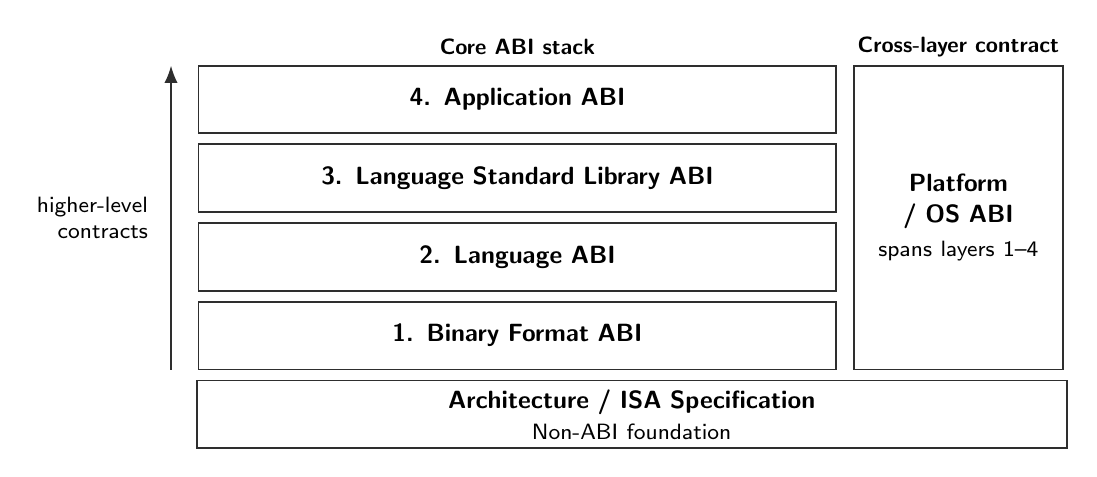
\begin{tikzpicture}[
    bedrockContract/.style={draw=RuleGray,fill=white,line width=0.65pt,minimum height=0.86cm,inner ysep=0pt,align=center,font=\small},
    bedrockCoreLayer/.style={bedrockContract,minimum width=8.10cm,text width=7.65cm},
    bedrockPlatformSpan/.style={bedrockContract,minimum width=2.65cm,minimum height=3.86cm,text width=2.25cm},
    bedrockFoundation/.style={bedrockContract,minimum width=11.05cm,text width=10.60cm},
    bedrockCurrentContract/.style={draw=black,fill=black!20,line width=1.25pt},
    bedrockLayerAxis/.style={-{Latex[length=2.2mm,width=1.7mm]},draw=RuleGray,line width=0.65pt}
  ]
  \node[font=\footnotesize\bfseries] at (-1.55,4.82) {Core ABI stack};
  \node[font=\footnotesize\bfseries] at (4.05,4.82) {Cross-layer contract};
  \BedrockContractNode{application}{bedrockCoreLayer}{application}{(-1.55,4.15)}{\textbf{4. Application ABI}}
  \BedrockContractNode{standard-library}{bedrockCoreLayer}{standardlibrary}{(-1.55,3.15)}{\textbf{3. Language Standard Library ABI}}
  \BedrockContractNode{language}{bedrockCoreLayer}{language}{(-1.55,2.15)}{\textbf{2. Language ABI}}
  \BedrockContractNode{binary}{bedrockCoreLayer}{binary}{(-1.55,1.15)}{\textbf{1. Binary Format ABI}}
  \BedrockContractNode{platform}{bedrockPlatformSpan}{platform}{(4.05,2.65)}{\textbf{Platform / OS ABI}\\[0.5mm]{\footnotesize spans layers 1--4}}
  \BedrockContractNode{foundation}{bedrockFoundation}{foundation}{(-0.10,0.15)}{\textbf{Architecture / ISA Specification}\\{\footnotesize Non-ABI foundation}}
  \draw[bedrockLayerAxis] (-5.95,0.72) -- (-5.95,4.58);
  \node[font=\footnotesize,align=right,anchor=east] at (-6.12,2.65) {higher-level\\contracts};
  \end{tikzpicture}
  \end{center}
  \noindent\footnotesize\textbf{Current document:} \BedrockDocumentTitle. The shaded block identifies its primary contract position. The Platform / OS ABI spans and constrains the four core ABI layers; the ISA specification is their non-ABI architectural foundation.\normalsize\par}
